\documentclass[11pt, letterpaper]{article}

% Fonts and Encoding
\usepackage[utf8]{inputenc}
\usepackage[T1]{fontenc}
\usepackage{lmodern} % High-quality Latin Modern vector font

% Math and Symbols
\usepackage{amsmath, amssymb, amsthm, amsfonts, mathrsfs, mathtools}

% Layout and Geometry
\usepackage{geometry}
\geometry{letterpaper, margin=1in}
\setlength{\parindent}{0pt}
\setlength{\parskip}{0.6em}

% Formatting and Graphics
\usepackage{graphicx, xcolor, enumitem, booktabs, array, tabularx}

% TikZ for Illustrations
\usepackage{tikz}
\usetikzlibrary{arrows.meta, positioning, shapes.geometric, calc, backgrounds, matrix}

% Clickable Links and TOC
\usepackage{hyperref}
\hypersetup{
    colorlinks=true,
    linkcolor=blue,
    filecolor=magenta,      
    urlcolor=cyan,
    pdftitle={Advanced Mathematics Topic},
}

% Theorem Environments
\newtheorem{theorem}{Theorem}[section]
\newtheorem{lemma}[theorem]{Lemma}
\newtheorem{proposition}[theorem]{Proposition}
\newtheorem{corollary}[theorem]{Corollary}
\theoremstyle{definition}
\newtheorem{definition}{Definition}[section]
\newtheorem{axiom}{Axiom}[section]
\newtheorem{example}{Example}[section]
\theoremstyle{remark}
\newtheorem{remark}{Remark}[section]

% Custom Commands (Enforced standard notation)
\newcommand{\R}{\mathbb{R}}
\newcommand{\N}{\mathbb{N}}
\newcommand{\Z}{\mathbb{Z}}
\newcommand{\Q}{\mathbb{Q}}
\newcommand{\E}{\mathbb{E}}
\newcommand{\Prob}{\mathbb{P}}
\newcommand{\F}{\mathcal{F}}

\begin{document}

\title{Mastering Composition of Functions: \\ Rigorous Practice Problem Set}
\author{Tashfeen Omran}
\date{November 12, 2026}
\maketitle

\tableofcontents
\newpage

\section{Concept Checklist \& Question Mapping}

The following table maps the theoretical concepts, logical structures, and proof techniques extracted from the source material to the 30 rigorous problems provided in this document.

\renewcommand{\arraystretch}{1.5}
\begin{tabularx}{\textwidth}{>{\bfseries}l X >{\bfseries}l}
\toprule
ID & Concept \& Logical Structure & Problems \\
\midrule
C1 & Direct Computation \& Algebraic Manipulation & 1, 2, 3, 4, 5 \\
C2 & Abstract Property Proofs: Injectivity \& Surjectivity & 6, 7, 8, 9, 10 \\
C3 & Abstract Property Proofs: Associativity \& Identity & 11, 12, 13 \\
C4 & Left and Right Inverses (Existence \& Implications) & 14, 15, 16, 17 \\
C5 & Counterexamples: Minimal Viable Sets \& Edge Cases & 18, 19, 20, 21, 22 \\
C6 & Systems of Linear Diophantine Equations in Mappings & 23, 24, 25 \\
C7 & Real-World Modeling: Deep Learning \& Chain Rule & 26, 27 \\
C8 & Real-World Modeling: Stochastic Matrices \& Markov & 28 \\
C9 & Functional Analysis \& Operator Composition & 29 \\
C10 & Advanced Diagnostic Testing: "Find the Flaw" & 30 \\
\bottomrule
\end{tabularx}

\newpage

\section{Problem Sets}

\subsection{Direct Computation \& Algebraic Manipulation}

\textbf{Problem 1.} Let $A = \{1, 2, 3, 4\}$, $B = \{a, b, c, d\}$, and $C = \{\alpha, \beta, \gamma\}$. Define $f: A \to B$ as $f = \{(1, c), (2, a), (3, d), (4, c)\}$ and $g: B \to C$ as $g = \{(a, \beta), (b, \gamma), (c, \alpha), (d, \beta)\}$. Determine the composition $g \circ f$ as a set of ordered pairs.

\textbf{Problem 2.} Consider the functions $f, g: \Z_{14} \to \Z_{14}$ defined by $f([x]) = [5x]$ and $g([x]) = [3x]$. Prove that $g \circ f = i_{\Z_{14}}$, where $i_{\Z_{14}}$ is the identity function on $\Z_{14}$.

\textbf{Problem 3.} The composition $(g \circ f): (0, \infty) \to \R$ is given by $(g \circ f)(x) = \frac{2x + 1}{x + 2}$. If $f(x) = x - 1$, determine the explicit algebraic formula for $g(x)$ and state its domain.

\textbf{Problem 4.} Let $f(x) = e^{2x}$ for $x \in \R$. Find a function $g: (0, \infty) \to \R$ such that $(f \circ g)(x) = x^4$ for all $x > 0$.

\textbf{Problem 5.} Let $f: \R \to \R$ and $g: \R \to \R$ be defined as follows:
\[
f(x) = 
\begin{cases} 
2x & \text{if } x < 0 \\ 
x^2 & \text{if } x \ge 0 
\end{cases}
\quad \text{and} \quad
g(x) = x - 3
\]
Determine the explicit piecewise definition of $(f \circ g)(x)$.

\subsection{Abstract Property Proofs: Injectivity \& Surjectivity}

\textbf{Problem 6.} Let $f: A \to B$ and $g: B \to C$ be functions. Prove rigorously that if $g \circ f$ is injective, then $f$ must be injective.

\textbf{Problem 7.} Let $f: A \to B$ and $g: B \to C$ be functions. Prove rigorously that if $g \circ f$ is surjective, then $g$ must be surjective.

\textbf{Problem 8.} Let $f: A \to B$ and $g: B \to C$ be functions. Prove that if $g \circ f$ is bijective, then $f$ is injective and $g$ is surjective.

\textbf{Problem 9.} Let $f: A \to B$ and $g: B \to C$. Prove by contradiction that if $f$ is surjective and $g$ is not injective, then $g \circ f$ cannot be injective.

\textbf{Problem 10.} Let $f: A \to B$ and $g: B \to A$. Prove that if $f \circ g = i_B$ and $g \circ f = i_A$, then $f$ is a bijection.

\subsection{Abstract Property Proofs: Associativity \& Identity}

\textbf{Problem 11.} Let $f: A \to B$, $g: B \to C$, and $h: C \to D$. Prove that function composition is associative; that is, $h \circ (g \circ f) = (h \circ g) \circ f$.

\textbf{Problem 12.} Let $f: A \to A$ be a function. Prove that if $f \circ f$ is injective, then $f$ is injective.

\textbf{Problem 13.} Let $f: A \to A$ be a function. Prove that if $f \circ f = f$ and $f$ is surjective, then $f = i_A$.

\subsection{Left and Right Inverses}

\textbf{Problem 14.} Let $f: A \to B$. Prove that if $f$ has a left inverse $g: B \to A$ (meaning $g \circ f = i_A$), then $f$ is injective.

\textbf{Problem 15.} Let $f: A \to B$. Prove that if $f$ has a right inverse $h: B \to A$ (meaning $f \circ h = i_B$), then $f$ is surjective.

\textbf{Problem 16.} Construct a concrete counterexample of a function $f: \N \to \N$ that has a left inverse but does not have a right inverse.

\textbf{Problem 17.} Let $f: A \to B$. Prove that if $f$ has a left inverse $g$ and a right inverse $h$, then $g = h$, and consequently $f$ is bijective.

\subsection{Counterexamples: Minimal Viable Sets \& Edge Cases}

\textbf{Problem 18.} Provide a minimal viable counterexample to disprove the following claim: "If $g \circ f$ is injective, then $g$ is injective."

\textbf{Problem 19.} Provide a minimal viable counterexample to disprove the following claim: "If $g \circ f$ is surjective, then $f$ is surjective."

\textbf{Problem 20.} Disprove the Commutative Fallacy by providing two functions $f, g: \R \to \R$ such that $f \circ g \neq g \circ f$.

\textbf{Problem 21.} A function $f: A \to A$ is called idempotent if $f \circ f = f$. Provide a counterexample to show that an idempotent function is not necessarily the identity function $i_A$.

\textbf{Problem 22.} Demonstrate a Domain Mismatch by defining two functions $f$ and $g$ such that $g \circ f$ is a well-defined function on $\R$, but $f \circ g$ is undefined for some $x \in \R$.

\subsection{Systems of Linear Diophantine Equations in Mappings}

\textbf{Problem 23.} Let $f: \Z \times \Z \to \Z \times \Z$ be defined by $f(a, b) = (2a + b, a + b)$. Determine if $f$ is surjective. If it is not, provide a specific element in $\Z \times \Z$ that has no pre-image.

\textbf{Problem 24.} Let $f: \R \times \R \to \R \times \R$ be defined by $f(x, y) = (2x + y, x - y)$ and $g: \R \times \R \to \R \times \R$ be defined by $g(u, v) = (u + v, u - 2v)$. Find the explicit formula for $(g \circ f)(x, y)$ and prove it is bijective.

\textbf{Problem 25.} Let $A$ be the set of even integers and $B$ be the set of odd integers. Let $f: A \times B \to \Z \times \Z$ be defined by $f(a, b) = (a + b, a - b)$. Let $g: \Z \times \Z \to \Z$ be defined by $g(x, y) = x^2 - y^2$. Evaluate $(g \circ f)(4, 3)$ and find a general simplified algebraic formula for $(g \circ f)(a, b)$.

\subsection{Real-World Modeling: Deep Learning \& Chain Rule}

\textbf{Problem 26.} In a 2-layer feedforward neural network, the mapping from input $x \in \R$ to output $y \in \R$ is given by $F(x) = (f_2 \circ f_1)(x)$. Let $f_1(x) = \sigma(w_1 x)$ and $f_2(h) = w_2 h$, where $\sigma(z) = \max(0, z)$ is the ReLU activation function. If $w_1 = -2$, $w_2 = 3$, and $x = -1$, compute $F(-1)$.

\textbf{Problem 27.} Let $\mathcal{L}(y, \hat{y}) = (y - \hat{y})^2$ be a loss function. Let $\hat{y} = F(x) = (f_2 \circ f_1)(x)$ where $f_1(x) = w_1 x$ and $f_2(h) = w_2 h$. Using the chain rule for function composition, derive the gradient $\frac{\partial \mathcal{L}}{\partial w_1}$ in terms of $x, y, w_1$, and $w_2$.

\subsection{Real-World Modeling: Stochastic Matrices \& Markov}

\textbf{Problem 28.} Let $S = \{1, 2\}$ be a state space. A Markov transition mapping $P: S \to \Delta(S)$ (where $\Delta(S)$ is the set of probability distributions over $S$) can be represented by a matrix. Let $f$ be the transition mapping represented by matrix $M_f = \begin{bmatrix} 0.8 & 0.2 \\ 0.4 & 0.6 \end{bmatrix}$. The composition $f \circ f$ represents a 2-step transition. Compute the matrix for $f \circ f$ and determine the probability of transitioning from state 1 to state 2 in exactly two steps.

\subsection{Functional Analysis \& Operator Composition}

\textbf{Problem 29.} Let $V$ be the vector space of infinitely differentiable functions from $\R$ to $\R$. Let $D: V \to V$ be the derivative operator defined by $D(f) = f'$. Let $M: V \to V$ be the multiplication operator defined by $M(f)(x) = x \cdot f(x)$. Prove that $(D \circ M)(f) - (M \circ D)(f) = f$ for all $f \in V$.

\subsection{Advanced Diagnostic Testing: "Find the Flaw"}

\textbf{Problem 30.} Identify the logical flaw in the following proof:
\textit{Claim:} Let $f: A \to B$ and $g: B \to C$. If $g \circ f$ is bijective, then $f$ is bijective.
\textit{Proof:} Assume $g \circ f$ is bijective. By definition, $g \circ f$ is both injective and surjective. Since $g \circ f$ is injective, by the Inner Rule, $f$ must be injective. Since $g \circ f$ is surjective, for every $c \in C$, there exists an $a \in A$ such that $g(f(a)) = c$. Let $b = f(a)$. This shows that $f$ maps elements of $A$ to elements of $B$ to cover the required inputs for $g$. Therefore, $f$ is surjective. Since $f$ is both injective and surjective, $f$ is bijective. $\blacksquare$

\newpage

\section{Detailed Solutions}

\textbf{Solution 1.}
We evaluate $g(f(x))$ for each $x \in A$:
\begin{align*}
(g \circ f)(1) &= g(f(1)) = g(c) = \alpha \\
(g \circ f)(2) &= g(f(2)) = g(a) = \beta \\
(g \circ f)(3) &= g(f(3)) = g(d) = \beta \\
(g \circ f)(4) &= g(f(4)) = g(c) = \alpha
\end{align*}
Expressing this as a set of ordered pairs:
\[
g \circ f = \{(1, \alpha), (2, \beta), (3, \beta), (4, \alpha)\}
\]
\qed

\textbf{Solution 2.}
We compute the composition using modular arithmetic in $\Z_{14}$. Let $[x] \in \Z_{14}$.
\[
(g \circ f)([x]) = g(f([x])) = g([5x]) = [3(5x)] = [15x]
\]
Since $15 \equiv 1 \pmod{14}$, we have $[15x] = [1x] = [x]$.
Thus, $(g \circ f)([x]) = [x]$ for all $[x] \in \Z_{14}$, which means $g \circ f = i_{\Z_{14}}$.
\qed

\textbf{Solution 3.}
We are given $g(f(x)) = \frac{2x + 1}{x + 2}$ and $f(x) = x - 1$. 
Let $u = f(x) = x - 1$. We solve for $x$ in terms of $u$:
\[
x = u + 1
\]
Substitute $x = u + 1$ into the expression for $g(f(x))$:
\[
g(u) = \frac{2(u + 1) + 1}{(u + 1) + 2} = \frac{2u + 2 + 1}{u + 3} = \frac{2u + 3}{u + 3}
\]
Thus, $g(x) = \frac{2x + 3}{x + 3}$. The domain of $g$ is $\R \setminus \{-3\}$.
\qed

\textbf{Solution 4.}
We are given $f(g(x)) = x^4$ and $f(x) = e^{2x}$.
Substitute $g(x)$ into $f$:
\[
f(g(x)) = e^{2g(x)}
\]
Set this equal to $x^4$:
\[
e^{2g(x)} = x^4
\]
Take the natural logarithm of both sides (valid since $x > 0 \implies x^4 > 0$):
\[
2g(x) = \ln(x^4) = 4\ln(x)
\]
Divide by 2:
\[
g(x) = 2\ln(x)
\]
\qed

\textbf{Solution 5.}
We need to evaluate $f(g(x)) = f(x - 3)$. The piecewise condition for $f$ depends on whether its input is less than 0 or greater than/equal to 0. The input to $f$ is $x - 3$.
Case 1: $x - 3 < 0 \implies x < 3$.
In this case, $f(x - 3) = 2(x - 3) = 2x - 6$.
Case 2: $x - 3 \ge 0 \implies x \ge 3$.
In this case, $f(x - 3) = (x - 3)^2 = x^2 - 6x + 9$.
Therefore, the explicit piecewise definition is:
\[
(f \circ g)(x) = 
\begin{cases} 
2x - 6 & \text{if } x < 3 \\ 
x^2 - 6x + 9 & \text{if } x \ge 3 
\end{cases}
\]
\qed

\textbf{Solution 6.}
\textit{Proof.} Assume $g \circ f: A \to C$ is injective. We must show $f: A \to B$ is injective. Let $x_1, x_2 \in A$ and assume $f(x_1) = f(x_2)$. 
Apply the function $g$ to both sides:
\[
g(f(x_1)) = g(f(x_2))
\]
By definition of composition, this is:
\[
(g \circ f)(x_1) = (g \circ f)(x_2)
\]
Since $g \circ f$ is injective, this implies $x_1 = x_2$. Therefore, $f$ is injective.
\qed

\textbf{Solution 7.}
\textit{Proof.} Assume $g \circ f: A \to C$ is surjective. We must show $g: B \to C$ is surjective. Let $c \in C$ be an arbitrary element. 
Since $g \circ f$ is surjective, there exists an element $a \in A$ such that:
\[
(g \circ f)(a) = c \implies g(f(a)) = c
\]
Let $b = f(a)$. Since $f: A \to B$, we know $b \in B$. Substituting $b$ into the equation yields $g(b) = c$. 
Thus, for every $c \in C$, there exists a $b \in B$ such that $g(b) = c$. Therefore, $g$ is surjective.
\qed

\textbf{Solution 8.}
\textit{Proof.} Assume $g \circ f$ is bijective. By definition, $g \circ f$ is both injective and surjective.
1. Since $g \circ f$ is injective, by the result of Problem 6, $f$ is injective.
2. Since $g \circ f$ is surjective, by the result of Problem 7, $g$ is surjective.
Therefore, $f$ is injective and $g$ is surjective.
\qed

\textbf{Solution 9.}
\textit{Proof.} Assume for the sake of contradiction that $f$ is surjective, $g$ is not injective, but $g \circ f$ is injective.
Since $g$ is not injective, there exist $b_1, b_2 \in B$ with $b_1 \neq b_2$ such that $g(b_1) = g(b_2)$.
Since $f$ is surjective, there exist $a_1, a_2 \in A$ such that $f(a_1) = b_1$ and $f(a_2) = b_2$. 
Because $b_1 \neq b_2$, it must be that $a_1 \neq a_2$ (otherwise $f$ would not be a well-defined function).
Now, evaluate $g \circ f$ at $a_1$ and $a_2$:
\[
(g \circ f)(a_1) = g(f(a_1)) = g(b_1)
\]
\[
(g \circ f)(a_2) = g(f(a_2)) = g(b_2)
\]
Since $g(b_1) = g(b_2)$, we have $(g \circ f)(a_1) = (g \circ f)(a_2)$. 
However, $a_1 \neq a_2$. This means $g \circ f$ is not injective, which contradicts our assumption that $g \circ f$ is injective. Thus, $g \circ f$ cannot be injective.
\qed

\textbf{Solution 10.}
\textit{Proof.} We are given $f \circ g = i_B$ and $g \circ f = i_A$.
First, we show $f$ is injective. Let $x_1, x_2 \in A$ and assume $f(x_1) = f(x_2)$. Apply $g$ to both sides:
\[
g(f(x_1)) = g(f(x_2)) \implies (g \circ f)(x_1) = (g \circ f)(x_2)
\]
Since $g \circ f = i_A$, this reduces to $i_A(x_1) = i_A(x_2) \implies x_1 = x_2$. Thus, $f$ is injective.
Next, we show $f$ is surjective. Let $y \in B$. We must find an $x \in A$ such that $f(x) = y$. Let $x = g(y)$. Since $g: B \to A$, $x \in A$. Evaluate $f(x)$:
\[
f(x) = f(g(y)) = (f \circ g)(y) = i_B(y) = y
\]
Thus, $f$ is surjective. Since $f$ is both injective and surjective, it is a bijection.
\qed

\textbf{Solution 11.}
\textit{Proof.} Let $x \in A$ be an arbitrary element. We evaluate the left side of the equation:
\[
(h \circ (g \circ f))(x) = h((g \circ f)(x)) = h(g(f(x)))
\]
Now we evaluate the right side of the equation:
\[
((h \circ g) \circ f)(x) = (h \circ g)(f(x)) = h(g(f(x)))
\]
Since $(h \circ (g \circ f))(x) = ((h \circ g) \circ f)(x)$ for all $x \in A$, the functions are equal.
\qed

\textbf{Solution 12.}
\textit{Proof.} Assume $f \circ f$ is injective. We must show $f$ is injective. Let $x_1, x_2 \in A$ and assume $f(x_1) = f(x_2)$. 
Since $f$ is a well-defined function, applying $f$ to both sides preserves equality:
\[
f(f(x_1)) = f(f(x_2))
\]
By definition of composition, this is:
\[
(f \circ f)(x_1) = (f \circ f)(x_2)
\]
Since $f \circ f$ is injective, this implies $x_1 = x_2$. Therefore, $f$ is injective.
\qed

\textbf{Solution 13.}
\textit{Proof.} Assume $f \circ f = f$ and $f$ is surjective. Let $x \in A$ be an arbitrary element. Since $f$ is surjective, there exists a $y \in A$ such that $f(y) = x$. 
We are given $(f \circ f)(y) = f(y)$ for all $y \in A$. 
Substitute $f(y) = x$ into the equation:
\[
f(f(y)) = f(y) \implies f(x) = x
\]
Since $f(x) = x$ for all $x \in A$, $f$ is the identity function $i_A$.
\qed

\textbf{Solution 14.}
\textit{Proof.} Assume $f: A \to B$ has a left inverse $g: B \to A$, so $g \circ f = i_A$. We must show $f$ is injective. Let $x_1, x_2 \in A$ and assume $f(x_1) = f(x_2)$. Apply $g$ to both sides:
\[
g(f(x_1)) = g(f(x_2)) \implies (g \circ f)(x_1) = (g \circ f)(x_2)
\]
Since $g \circ f = i_A$, this yields $i_A(x_1) = i_A(x_2) \implies x_1 = x_2$. Thus, $f$ is injective.
\qed

\textbf{Solution 15.}
\textit{Proof.} Assume $f: A \to B$ has a right inverse $h: B \to A$, so $f \circ h = i_B$. We must show $f$ is surjective. Let $y \in B$ be an arbitrary element. We need to find an $x \in A$ such that $f(x) = y$. 
Let $x = h(y)$. Since $h: B \to A$, $x \in A$. Evaluate $f(x)$:
\[
f(x) = f(h(y)) = (f \circ h)(y) = i_B(y) = y
\]
Since we found an $x \in A$ for every $y \in B$, $f$ is surjective.
\qed

\textbf{Solution 16.}
Let $f: \N \to \N$ be defined by $f(n) = n + 1$. 
Define $g: \N \to \N$ as:
\[
g(n) = 
\begin{cases} 
n - 1 & \text{if } n > 1 \\ 
1 & \text{if } n = 1 
\end{cases}
\]
We check if $g$ is a left inverse. $(g \circ f)(n) = g(n + 1)$. Since $n \ge 1$, $n + 1 \ge 2 > 1$, so $g(n + 1) = (n + 1) - 1 = n$. Thus, $g \circ f = i_\N$, so $g$ is a left inverse.
However, $f$ is not surjective (1 has no pre-image). By the contrapositive of Problem 15, since $f$ is not surjective, it cannot have a right inverse.

\begin{center}
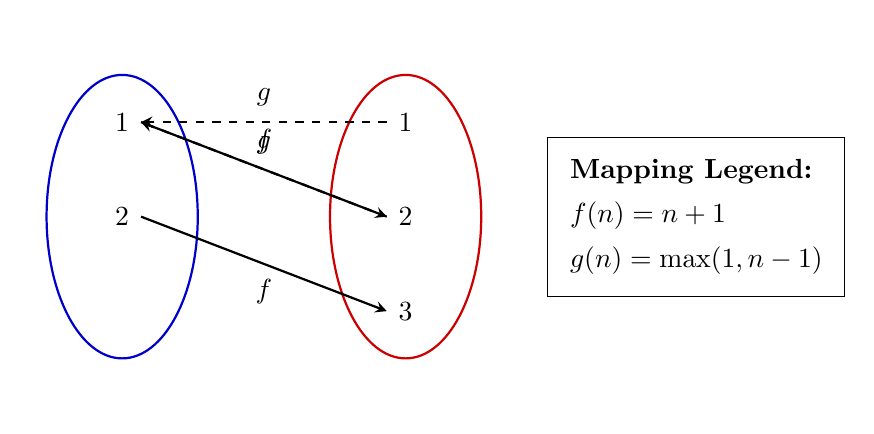
\begin{tikzpicture}[scale=1.2]
\fill[white] (-1,-1) rectangle (5,3); % Background
% Draw sets
\draw[thick, blue!80!black] (0,1) ellipse (0.8 and 1.5);
\draw[thick, red!80!black] (3,1) ellipse (0.8 and 1.5);
% Nodes
\node[align=left] at (0, 2) {$1$};
\node[align=left] at (0, 1) {$2$};
\node[align=left] at (3, 2) {$1$};
\node[align=left] at (3, 1) {$2$};
\node[align=left] at (3, 0) {$3$};
% Arrows
\draw[->, >=stealth, thick] (0.2, 2) -- (2.8, 1) node[midway, above=2pt] {$f$};
\draw[->, >=stealth, thick] (0.2, 1) -- (2.8, 0) node[midway, below=2pt] {$f$};
\draw[->, >=stealth, thick, dashed] (2.8, 1) -- (0.2, 2) node[midway, above=2pt] {$g$};
\draw[->, >=stealth, thick, dashed] (2.8, 2) -- (0.2, 2) node[midway, above=2pt] {$g$};
% Legend
\node[align=left, anchor=west, draw, inner sep=8pt] at (4.5, 1) {
    \textbf{Mapping Legend:}\\[4pt]
    $f(n) = n+1$\\[4pt]
    $g(n) = \max(1, n-1)$
};
\end{tikzpicture}
\end{center}
\qed

\textbf{Solution 17.}
\textit{Proof.} We are given $g \circ f = i_A$ and $f \circ h = i_B$. We use the associativity of function composition (Problem 11).
Consider the composition $g \circ f \circ h$. We can group this in two ways:
\[
g \circ (f \circ h) = g \circ i_B = g
\]
\[
(g \circ f) \circ h = i_A \circ h = h
\]
Since composition is associative, $g \circ (f \circ h) = (g \circ f) \circ h$. Therefore, $g = h$. 
Since $f$ has a left inverse, it is injective. Since it has a right inverse, it is surjective. Thus, $f$ is bijective, and $g = h = f^{-1}$.
\qed

\textbf{Solution 18.}
Let $A = \{1\}$, $B = \{1, 2\}$, and $C = \{1\}$. 
Define $f: A \to B$ by $f(1) = 1$. 
Define $g: B \to C$ by $g(1) = 1$ and $g(2) = 1$. 
The composition $g \circ f: A \to C$ maps $1 \mapsto 1$. Since $A$ has only one element, $g \circ f$ is trivially injective. 
However, $g(1) = g(2) = 1$ with $1 \neq 2$, so $g$ is not injective.
\qed

\textbf{Solution 19.}
Let $A = \{1\}$, $B = \{1, 2\}$, and $C = \{1\}$. 
Define $f: A \to B$ by $f(1) = 1$. 
Define $g: B \to C$ by $g(1) = 1$ and $g(2) = 1$. 
The composition $g \circ f: A \to C$ maps $1 \mapsto 1$. Since the image is $\{1\} = C$, $g \circ f$ is surjective. 
However, the image of $f$ is $\{1\} \neq B$, so $f$ is not surjective.
\qed

\textbf{Solution 20.}
Let $f(x) = x^2$ and $g(x) = x + 1$. 
Evaluate $(f \circ g)(x)$:
\[
(f \circ g)(x) = f(x + 1) = (x + 1)^2 = x^2 + 2x + 1
\]
Evaluate $(g \circ f)(x)$:
\[
(g \circ f)(x) = g(x^2) = x^2 + 1
\]
Since $x^2 + 2x + 1 \neq x^2 + 1$ for $x \neq 0$, $f \circ g \neq g \circ f$.
\qed

\textbf{Solution 21.}
Let $f: \R \to \R$ be defined by $f(x) = |x|$. 
Evaluate $(f \circ f)(x)$:
\[
(f \circ f)(x) = f(|x|) = ||x|| = |x| = f(x)
\]
Thus, $f \circ f = f$, making $f$ idempotent. However, $f(-2) = 2 \neq -2$, so $f$ is not the identity function $i_\R$.
\qed

\textbf{Solution 22.}
Let $f: \R \to [0, \infty)$ be defined by $f(x) = x^2$. 
Let $g: [0, \infty) \to \R$ be defined by $g(x) = \sqrt{x}$. 
The composition $(g \circ f)(x) = g(x^2) = \sqrt{x^2} = |x|$ is well-defined for all $x \in \R$. 
However, the composition $(f \circ g)(x) = f(\sqrt{x})$ requires the input to $g$ to be non-negative. If we attempt to evaluate $(f \circ g)(-1)$, $g(-1) = \sqrt{-1}$ is undefined in $\R$. Thus, $f \circ g$ is undefined on $\R$.
\qed

\textbf{Solution 23.}
To determine if $f$ is surjective, we set $f(a, b) = (x, y)$ for arbitrary $(x, y) \in \Z \times \Z$ and solve for $(a, b) \in \Z \times \Z$.
\begin{align*}
2a + b &= x \\
a + b &= y
\end{align*}
Subtracting the second equation from the first yields:
\[
a = x - y
\]
Substitute $a$ into the second equation:
\[
(x - y) + b = y \implies b = 2y - x
\]
Since $x, y \in \Z$, both $a = x - y$ and $b = 2y - x$ are integers. Thus, for any $(x, y) \in \Z \times \Z$, there exists a pre-image $(a, b) \in \Z \times \Z$. Therefore, $f$ is surjective.
\qed

\textbf{Solution 24.}
First, we find the explicit formula for $(g \circ f)(x, y)$:
\begin{align*}
(g \circ f)(x, y) &= g(2x + y, x - y) \\
&= ((2x + y) + (x - y), (2x + y) - 2(x - y)) \\
&= (3x, 2x + y - 2x + 2y) \\
&= (3x, 3y)
\end{align*}
To prove bijectivity, we show it is injective and surjective.
\textit{Injectivity:} Assume $(3x_1, 3y_1) = (3x_2, 3y_2)$. Then $3x_1 = 3x_2 \implies x_1 = x_2$ and $3y_1 = 3y_2 \implies y_1 = y_2$. Thus, it is injective.
\textit{Surjectivity:} Let $(u, v) \in \R \times \R$. We need $(3x, 3y) = (u, v)$. Setting $x = u/3$ and $y = v/3$, since $u, v \in \R$, $x, y \in \R$. Thus, it is surjective.
Since it is both injective and surjective, $g \circ f$ is bijective.
\qed

\textbf{Solution 25.}
First, evaluate $(g \circ f)(4, 3)$:
\[
f(4, 3) = (4 + 3, 4 - 3) = (7, 1)
\]
\[
g(7, 1) = 7^2 - 1^2 = 49 - 1 = 48
\]
Next, find the general formula:
\begin{align*}
(g \circ f)(a, b) &= g(a + b, a - b) \\
&= (a + b)^2 - (a - b)^2 \\
&= (a^2 + 2ab + b^2) - (a^2 - 2ab + b^2) \\
&= 4ab
\end{align*}
\qed

\textbf{Solution 26.}
We are given $x = -1$, $w_1 = -2$, and $w_2 = 3$.
First, compute the inner function $f_1(x)$:
\[
f_1(-1) = \sigma(-2(-1)) = \sigma(2) = \max(0, 2) = 2
\]
Next, compute the outer function $f_2(h)$ where $h = f_1(-1) = 2$:
\[
F(-1) = f_2(2) = 3(2) = 6
\]
\qed

\textbf{Solution 27.}
We have $\mathcal{L} = (y - \hat{y})^2$, $\hat{y} = w_2 h$, and $h = w_1 x$.
By the chain rule:
\[
\frac{\partial \mathcal{L}}{\partial w_1} = \frac{\partial \mathcal{L}}{\partial \hat{y}} \cdot \frac{\partial \hat{y}}{\partial h} \cdot \frac{\partial h}{\partial w_1}
\]
Compute each partial derivative:
\begin{align*}
\frac{\partial \mathcal{L}}{\partial \hat{y}} &= -2(y - \hat{y}) \\
\frac{\partial \hat{y}}{\partial h} &= w_2 \\
\frac{\partial h}{\partial w_1} &= x
\end{align*}
Multiply them together:
\[
\frac{\partial \mathcal{L}}{\partial w_1} = -2(y - \hat{y}) \cdot w_2 \cdot x
\]
Substitute $\hat{y} = w_2 w_1 x$:
\[
\frac{\partial \mathcal{L}}{\partial w_1} = -2x w_2 (y - w_1 w_2 x)
\]
\qed

\textbf{Solution 28.}
The composition of linear mappings represented by matrices is equivalent to matrix multiplication.
\[
M_{f \circ f} = M_f \times M_f = \begin{bmatrix} 0.8 & 0.2 \\ 0.4 & 0.6 \end{bmatrix} \begin{bmatrix} 0.8 & 0.2 \\ 0.4 & 0.6 \end{bmatrix}
\]
Compute the elements:
\begin{align*}
(1,1) &= 0.8(0.8) + 0.2(0.4) = 0.64 + 0.08 = 0.72 \\
(1,2) &= 0.8(0.2) + 0.2(0.6) = 0.16 + 0.12 = 0.28 \\
(2,1) &= 0.4(0.8) + 0.6(0.4) = 0.32 + 0.24 = 0.56 \\
(2,2) &= 0.4(0.2) + 0.6(0.6) = 0.08 + 0.36 = 0.44
\end{align*}
\[
M_{f \circ f} = \begin{bmatrix} 0.72 & 0.28 \\ 0.56 & 0.44 \end{bmatrix}
\]
The probability of transitioning from state 1 to state 2 in exactly two steps is the entry in row 1, column 2, which is $0.28$.
\qed

\textbf{Solution 29.}
\textit{Proof.} Let $f \in V$. We evaluate $(D \circ M)(f)$ and $(M \circ D)(f)$.
First, apply $M$ to $f$:
\[
M(f)(x) = x f(x)
\]
Now apply $D$ to $M(f)$. By the product rule:
\[
(D \circ M)(f)(x) = \frac{d}{dx}[x f(x)] = 1 \cdot f(x) + x \cdot f'(x) = f(x) + x f'(x)
\]
Next, evaluate $(M \circ D)(f)$. First apply $D$:
\[
D(f)(x) = f'(x)
\]
Now apply $M$:
\[
(M \circ D)(f)(x) = x f'(x)
\]
Subtract the two results:
\[
(D \circ M)(f)(x) - (M \circ D)(f)(x) = (f(x) + x f'(x)) - x f'(x) = f(x)
\]
Since this holds for all $x$, $(D \circ M)(f) - (M \circ D)(f) = f$.
\qed

\textbf{Solution 30.}
The flaw occurs in the deduction of surjectivity. The proof states: "Since $g \circ f$ is surjective, for every $c \in C$, there exists an $a \in A$ such that $g(f(a)) = c$. Let $b = f(a)$. This shows that $f$ maps elements of $A$ to elements of $B$ to cover the required inputs for $g$. Therefore, $f$ is surjective."
\textit{The Flaw:} This logic only proves that the image of $f$ covers the subset of $B$ necessary for $g$ to reach all of $C$. It does not prove that the image of $f$ covers \textit{all} of $B$. If there are elements in $B$ that $g$ maps redundantly to $C$, $f$ does not need to map to them for $g \circ f$ to be surjective. Thus, $f$ is not necessarily surjective, and therefore not necessarily bijective.
\qed

\newpage

\section{Concept Checklist \& Question Mapping (Repeated)}

\renewcommand{\arraystretch}{1.5}
\begin{tabularx}{\textwidth}{>{\bfseries}l X >{\bfseries}l}
\toprule
ID & Concept \& Logical Structure & Problems \\
\midrule
C1 & Direct Computation \& Algebraic Manipulation & 1, 2, 3, 4, 5 \\
C2 & Abstract Property Proofs: Injectivity \& Surjectivity & 6, 7, 8, 9, 10 \\
C3 & Abstract Property Proofs: Associativity \& Identity & 11, 12, 13 \\
C4 & Left and Right Inverses (Existence \& Implications) & 14, 15, 16, 17 \\
C5 & Counterexamples: Minimal Viable Sets \& Edge Cases & 18, 19, 20, 21, 22 \\
C6 & Systems of Linear Diophantine Equations in Mappings & 23, 24, 25 \\
C7 & Real-World Modeling: Deep Learning \& Chain Rule & 26, 27 \\
C8 & Real-World Modeling: Stochastic Matrices \& Markov & 28 \\
C9 & Functional Analysis \& Operator Composition & 29 \\
C10 & Advanced Diagnostic Testing: "Find the Flaw" & 30 \\
\bottomrule
\end{tabularx}

\end{document}